\def\layersep{1.5cm}
\def\outsep{0.7cm}
\def\dy{1.25}

\begin{tikzpicture}[draw=black!50, node distance=\layersep, font=\sffamily]
    \tikzstyle{node}=[circle,fill=black,minimum size=2pt,inner sep=0pt]
    \tikzstyle{block}=[draw=black,rectangle,fill=none,minimum size=1.5cm, inner sep=0pt]
    \tikzstyle{annot} = []

	\node[node] (xc) at (0, -\dy cm) {};
	
    \onslide<1|handout:1>{\node[block, text width = 2cm, align= center] (CH) at (2*\layersep, -\dy cm) {Channel};}
    
    \onslide<2-|handout:2->{\node[block, text width = 2cm, align= center] (CH) at (2*\layersep, -\dy cm) {Bad Channel};}
    
	\coordinate (yc) at (4*\layersep, -\dy cm) {};
		
    \path[->, >=stealth, shorten >= 0pt] (xc) edge (CH);
    \path[->, >=stealth, shorten >= 0pt] (CH) edge (yc);
    
    \node[block, draw=none, above = 0.5mm of xc, scale=0.5] (tx_signal) {\resizebox{!}{!}{\begin{tikzpicture}
\begin{axis}[
width=4.52in,
height=3.56in,
scale only axis,
separate axis lines,
every outer x axis line/.append style={white!15!black},
every x tick label/.append style={font=\color{white!15!black}},
xmin=0.00,
xmax=70.00,
ymin=0.00,
ymax=1.00,
xlabel={},
ylabel={},
xmajorgrids,
ymajorgrids,
every outer y axis line/.append style={white!15!black},
every y tick label/.append style={font=\color{white!15!black}},
legend style={draw=white!15!black,fill=white,legend cell align=left}]
\definecolor{matlabColor1}{rgb}{0.000000,0.447000,0.741000}
\addplot [color=matlabColor1, solid, line width=1.5pt, forget plot]
table[row sep=crcr]{
	1 0 \\
	2 0 \\
	3 0 \\
	4 0 \\
	5 0 \\
	6 0 \\
	7 0 \\
	8 0 \\
	9 0 \\
	10 0 \\
	11 0 \\
	12 1 \\
	13 1 \\
	14 1 \\
	15 1 \\
	16 1 \\
	17 1 \\
	18 1 \\
	19 1 \\
	20 1 \\
	21 1 \\
	22 1 \\
	23 0 \\
	24 0 \\
	25 0 \\
	26 0 \\
	27 0 \\
	28 0 \\
	29 0 \\
	30 0 \\
	31 0 \\
	32 0 \\
	33 0 \\
	34 1 \\
	35 1 \\
	36 1 \\
	37 1 \\
	38 1 \\
	39 1 \\
	40 1 \\
	41 1 \\
	42 1 \\
	43 1 \\
	44 1 \\
	45 1 \\
	46 1 \\
	47 1 \\
	48 1 \\
	49 1 \\
	50 1 \\
	51 1 \\
	52 1 \\
	53 1 \\
	54 1 \\
	55 1 \\
	56 0 \\
	57 0 \\
	58 0 \\
	59 0 \\
	60 0 \\
	61 0 \\
	62 0 \\
	63 0 \\
	64 0 \\
	65 0 \\
	66 0 \\
};

\end{axis}
\end{tikzpicture}}};
    \onslide<1|handout:1>\node[block, draw=none, above = 0.5mm of yc, scale=0.5] (tx_signal) {\resizebox{!}{!}{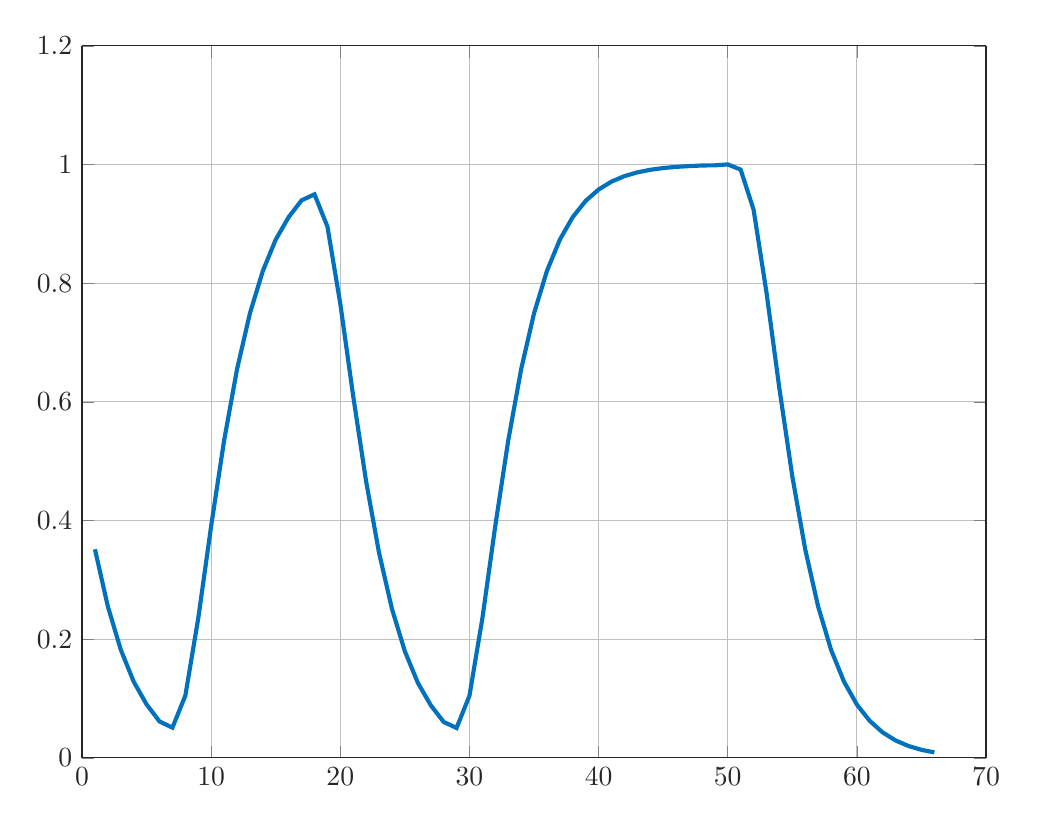
\begin{tikzpicture}
\begin{axis}[
width=4.52in,
height=3.56in,
scale only axis,
separate axis lines,
every outer x axis line/.append style={white!15!black},
every x tick label/.append style={font=\color{white!15!black}},
xmin=0.00,
xmax=70.00,
ymin=0.00,
ymax=1.20,
xlabel={},
ylabel={},
xmajorgrids,
ymajorgrids,
every outer y axis line/.append style={white!15!black},
every y tick label/.append style={font=\color{white!15!black}},
legend style={draw=white!15!black,fill=white,legend cell align=left}]
\definecolor{matlabColor1}{rgb}{0.000000,0.447000,0.741000}
\addplot [color=matlabColor1, solid, line width=1.5pt, forget plot]
table[row sep=crcr]{
	1 0.35141 \\
	2 0.25498 \\
	3 0.18215 \\
	4 0.12838 \\
	5 0.089941 \\
	6 0.06127 \\
	7 0.050858 \\
	8 0.10489 \\
	9 0.23518 \\
	10 0.39096 \\
	11 0.5346 \\
	12 0.65469 \\
	13 0.7491 \\
	14 0.82058 \\
	15 0.87344 \\
	16 0.91127 \\
	17 0.93953 \\
	18 0.94968 \\
	19 0.89546 \\
	20 0.76505 \\
	21 0.60919 \\
	22 0.4655 \\
	23 0.34537 \\
	24 0.25094 \\
	25 0.17945 \\
	26 0.12658 \\
	27 0.08874 \\
	28 0.060478 \\
	29 0.050327 \\
	30 0.10455 \\
	31 0.23495 \\
	32 0.39082 \\
	33 0.53449 \\
	34 0.65464 \\
	35 0.74903 \\
	36 0.8206 \\
	37 0.87333 \\
	38 0.91149 \\
	39 0.93866 \\
	40 0.95781 \\
	41 0.97113 \\
	42 0.98037 \\
	43 0.98669 \\
	44 0.99104 \\
	45 0.99395 \\
	46 0.99598 \\
	47 0.99725 \\
	48 0.99829 \\
	49 0.99857 \\
	50 1.0001 \\
	51 0.99134 \\
	52 0.92397 \\
	53 0.78446 \\
	54 0.62233 \\
	55 0.47438 \\
	56 0.35133 \\
	57 0.25497 \\
	58 0.18208 \\
	59 0.12846 \\
	60 0.089692 \\
	61 0.062127 \\
	62 0.042717 \\
	63 0.029214 \\
	64 0.01986 \\
	65 0.01346 \\
	66 0.0090624 \\
};

\end{axis}
\end{tikzpicture}}};
    \onslide<2-|handout:2->\node[block, draw=none, above = 0.5mm of yc, scale=0.5] (tx_signal) {\resizebox{!}{!}{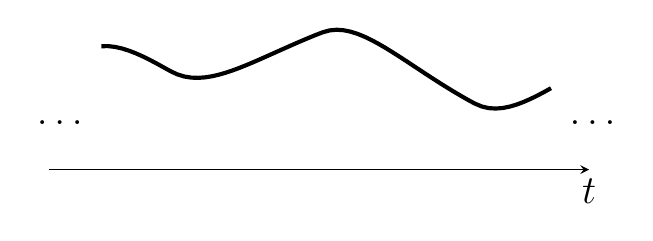
\begin{tikzpicture}
\begin{axis}[
axis lines*=middle,
enlargelimits = true,
hide y axis,
axis line style={->,>=stealth},
xmin=0.00,
xmax= 65.00,
ymin=0.00,
ymax=2.00,
clip=false,
xlabel={\Large $t$},
ylabel={},
xtick=\empty,
ytick=\empty,
every axis x label/.style={
	at={(ticklabel* cs:1)},
	anchor=north,
},
]
\node at (axis cs: 72, 0.25) {\Large$\ldots$};
\node at (axis cs: -5, 0.25) {\Large$\ldots$};
\addplot [color=black, solid, line width=1.5pt, forget plot]
table[row sep=crcr]{
	1 0.6606 \\
	2 0.66119 \\
	3 0.65685 \\
	4 0.64848 \\
	5 0.63679 \\
	6 0.6224 \\
	7 0.60585 \\
	8 0.58762 \\
	9 0.56813 \\
	10 0.54763 \\
	11 0.52712 \\
	12 0.50985 \\
	13 0.49845 \\
	14 0.49258 \\
	15 0.49132 \\
	16 0.49395 \\
	17 0.4998 \\
	18 0.50832 \\
	19 0.519 \\
	20 0.53142 \\
	21 0.5452 \\
	22 0.56002 \\
	23 0.57562 \\
	24 0.59174 \\
	25 0.60818 \\
	26 0.62478 \\
	27 0.64139 \\
	28 0.65789 \\
	29 0.67417 \\
	30 0.69016 \\
	31 0.70577 \\
	32 0.72103 \\
	33 0.73522 \\
	34 0.7453 \\
	35 0.74884 \\
	36 0.74634 \\
	37 0.73887 \\
	38 0.72727 \\
	39 0.7123 \\
	40 0.69462 \\
	41 0.67481 \\
	42 0.65334 \\
	43 0.63065 \\
	44 0.60709 \\
	45 0.58298 \\
	46 0.55858 \\
	47 0.53412 \\
	48 0.50978 \\
	49 0.48573 \\
	50 0.46207 \\
	51 0.43893 \\
	52 0.41638 \\
	53 0.39451 \\
	54 0.37328 \\
	55 0.35341 \\
	56 0.33794 \\
	57 0.32928 \\
	58 0.32694 \\
	59 0.32982 \\
	60 0.33708 \\
	61 0.34795 \\
	62 0.36176 \\
	63 0.37793 \\
	64 0.39597 \\
	65 0.41544 \\
	66 0.43596 \\
};

\end{axis}
\end{tikzpicture}}};

\end{tikzpicture}